\chapter{Contexte général}
\label{chap:premierchapitre}
\section*{Introduction du chapitre}
Ce chapitre présente le contexte général du projet ainsi que son cadre global. Il introduit d’abord l’organisme d’accueil DECADE Tunisie ainsi que son client ETANCO, avant de détailler les concepts fondamentaux liés à la gestion des informations des produits.

Nous analysons ensuite le contexte du projet et l’étude de l’existant afin de mettre en lumière la problématique identifiée. Enfin, nous présentons la solution proposée ainsi que la méthodologie Agile Scrum adoptée pour structurer le déroulement de ce travail.
\section{Présentation de l’organisme d’accueil}

Dans cette section, nous présentons l'organisme d'accueil, le client concerné par le projet, ainsi que les principaux domaines dans lesquels ils exercent leurs activités.

\subsection{Présentation de l’entreprise : DECADE}

DECADE est une Entreprise de Services du Numérique (ESN) spécialisée dans le conseil et la réalisation de solutions e-commerce et de transformation digitale. Depuis sa création en 1988, elle s’est imposée comme un partenaire stratégique pour les entreprises souhaitant titulariser leur activité commerciale en ligne.

L’expertise de DECADE repose sur une maîtrise approfondie des outils de vente en ligne, notamment SAP Commerce Cloud et sur une forte capacité à intégrer des problématiques complexes de gestion des informations des produits. L'entreprise accompagne ses clients tout au long du cycle de vie de leurs projets, de la conception logicielle à l'optimisation continue, en mettant l'accent sur la qualité des contenus et l'efficacité des processus métier.

Cette spécialisation dans le commerce électronique à forte valeur ajoutée constitue le cadre idéal pour ce projet de fin d'études, qui s'articule autour de l'amélioration du parcours d'enrichissement des informations des produits pour un client industriel majeur. L'identité visuelle de l'entreprise est illustrée par la Figure~\ref{fig:logo_decade}.

\begin{figure}[H]
    \centering
    
\includegraphics[width=0.2\textwidth]{images/logo_decade.png}
    \caption{Logo de DECADE}
    \label{fig:logo_decade}
\end{figure}

\subsection{Types de projets}

DECADE accompagne ses clients à travers des solutions adaptées à leurs objectifs stratégiques. Les principaux axes d’intervention de l’entreprise sont :

\begin{itemize}
    \item \textbf{Solutions e-commerce :} conception et développement de plateformes de vente robustes et évolutives.
    \item \textbf{Gestion des informations des produits (PIM/PXM) :} mise en place de référentiels uniques pour centraliser et enrichir les données des produits.
    \item \textbf{Expérience utilisateur (UX/UI) :} création de parcours d'achat ergonomiques et performants adaptés aux besoins des clients.
    \item \textbf{Marketplaces :} déploiement de solutions permettant d'étendre l'offre commerciale via des écosystèmes multipartenaires.
    \item \textbf{Gestion de la relation client (CRM) :} intégration d'outils de suivi et de fidélisation pour une meilleure connaissance du client.
    \item \textbf{Architectures API-first et Cloud :} mise en œuvre de systèmes modulaires et flexibles facilitant l'interopérabilité entre les outils.
\end{itemize}

\subsection{Présentation du client : ETANCO}

Dans le cadre de ce projet, DECADE intervient pour le compte d'ETANCO, une filiale du groupe international Simpson Strong-Tie. ETANCO est un acteur majeur en Europe dans la conception, la fabrication et la distribution de solutions de fixation et d'assemblage destinées à l'enveloppe du bâtiment. L'entreprise intervient dans plusieurs domaines, notamment la toiture, la façade, le bardage et l'étanchéité et s'adresse principalement aux professionnels du bâtiment.

Afin de répondre aux besoins de ses clients, ETANCO commercialise un catalogue comprenant plusieurs dizaines de milliers de références. Chaque produit est associé à de nombreuses informations, telles que des caractéristiques techniques, des descriptions, des documents réglementaires, des médias, des classifications ainsi que des traductions destinées aux différents marchés. La qualité, la cohérence et la disponibilité de ces informations sont essentielles pour assurer une présentation fiable des produits sur les différents canaux de diffusion de l'entreprise. La Figure~\ref{fig:logo_etanco} présente l'identité visuelle du groupe.

\begin{figure}[H]
    \centering
    
\includegraphics[width=0.2\textwidth]{images/etanco.jpg}
    \caption{Logo d'ETANCO}
    \label{fig:logo_etanco}
\end{figure}

\section{Concepts de base}

Cette section introduit les notions fondamentales nécessaires à la compréhension de la circulation des informations au sein d'une interface de vente moderne.

\subsection{Le commerce électronique}

Le commerce électronique, ou e-commerce, désigne l'échange de biens, de services ou d'informations par l'intermédiaire de réseaux informatiques, principalement Internet \cite{ibm_ecommerce}. Il ne se limite pas à l'acte d'achat, mais englobe l'ensemble du parcours client numérique.

On distingue généralement deux modèles principaux selon la nature des acteurs impliqués :

\begin{itemize}
    \item \textbf{B2C (Business-to-Consumer) :} les entreprises vendent directement aux particuliers. Le processus de décision est souvent court et émotionnel.
    \item \textbf{B2B (Business-to-Business) :} les échanges s'effectuent entre deux entités morales. Ce modèle, propre au contexte d'ETANCO, se caractérise par des catalogues complexes et des processus d'achat rationnels.
\end{itemize}

Le tableau \ref{tab:b2b_b2c} synthétise les disparités majeures entre ces deux approches.

\begin{table}[H]
    \centering
    \begin{tabular}{|l|p{6cm}|p{6cm}|}
    \hline
    \textbf{Caractéristique} & \textbf{E-commerce B2C} & \textbf{E-commerce B2B} \\ \hline
    \textbf{Client cible} & Particulier (Individu) & Professionnel (Entreprise) \\ \hline
    \textbf{Processus d'achat} & Rapide et impulsionnel & Long, structuré et validé \\ \hline
    \textbf{Volume / Prix} & Unitaire / Prix fixe & Quantités importantes / Prix négociés \\ \hline
    \textbf{Relation client} & Ponctuelle et court terme & Partenariale et pérenne \\ \hline
    \textbf{Catalogue} & Standardisé & Complexe et technique \\ \hline
    \end{tabular}
    \caption{Comparaison entre les modèles e-commerce B2B et B2C}
    \label{tab:b2b_b2c}
\end{table}
Cette comparaison met en évidence les différences fondamentales entre les deux approches e-commerce. Dans le contexte d'ETANCO, le modèle B2B prédomine : les clients sont des professionnels du bâtiment qui nécessitent des informations techniques précises, des catalogs complets et des relations commerciales structurées. Cette spécificité impose des exigences particulières en termes de qualité et d'exactitude des données des produits.
Une plateforme e-commerce s'appuie structurellement sur deux composantes :
\begin{itemize}
    \item \textbf{Front Office (Storefront) :} l'interface publique destinée aux utilisateurs pour la navigation et l'acquisition de produits.
    \item \textbf{Back Office :} l'interface d'administration permettant de gérer les catalogues, les commandes et les clients.
\end{itemize}

\subsection{Les systèmes intervenant dans le commerce électronique}

La gestion efficace d'une boutique en ligne repose sur l'interopérabilité de plusieurs logiciels métiers spécialisés :

\begin{itemize}
    \item \textbf{ERP (Enterprise Resource Planning) :} colonne vertébrale de l'entreprise, il centralise les données opérationnelles telles que les stocks, les tarifs et la comptabilité \cite{sap_erp}.
    \item \textbf{PIM (Product Information Management) :} référentiel unique dédié à la centralisation, l'enrichissement et la traduction des caractéristiques techniques et commerciales des produits \cite{akeneo_pim}.
    \item \textbf{SAP Commerce Cloud :} plateforme cloud omnicanale qui orchestre l'expérience client et le pilotage des processus de vente complexes \cite{sap_commerce_cloud}.
    \item \textbf{CRM (Customer Relationship Management) :} outil de gestion de la relation client permettant de suivre les interactions et d'optimiser les stratégies de fidélisation \cite{salesforce_crm}.
\end{itemize}

\subsection{Cycle de vie des données d'un produit}

Pour garantir la pertinence de l'offre en ligne, les informations des produits suivent un cycle de vie structuré à travers les différents systèmes. L'architecture technique de ce flux est illustrée dans la Figure~\ref{fig:cycle_vie}.

\begin{figure}[H]
    \centering
    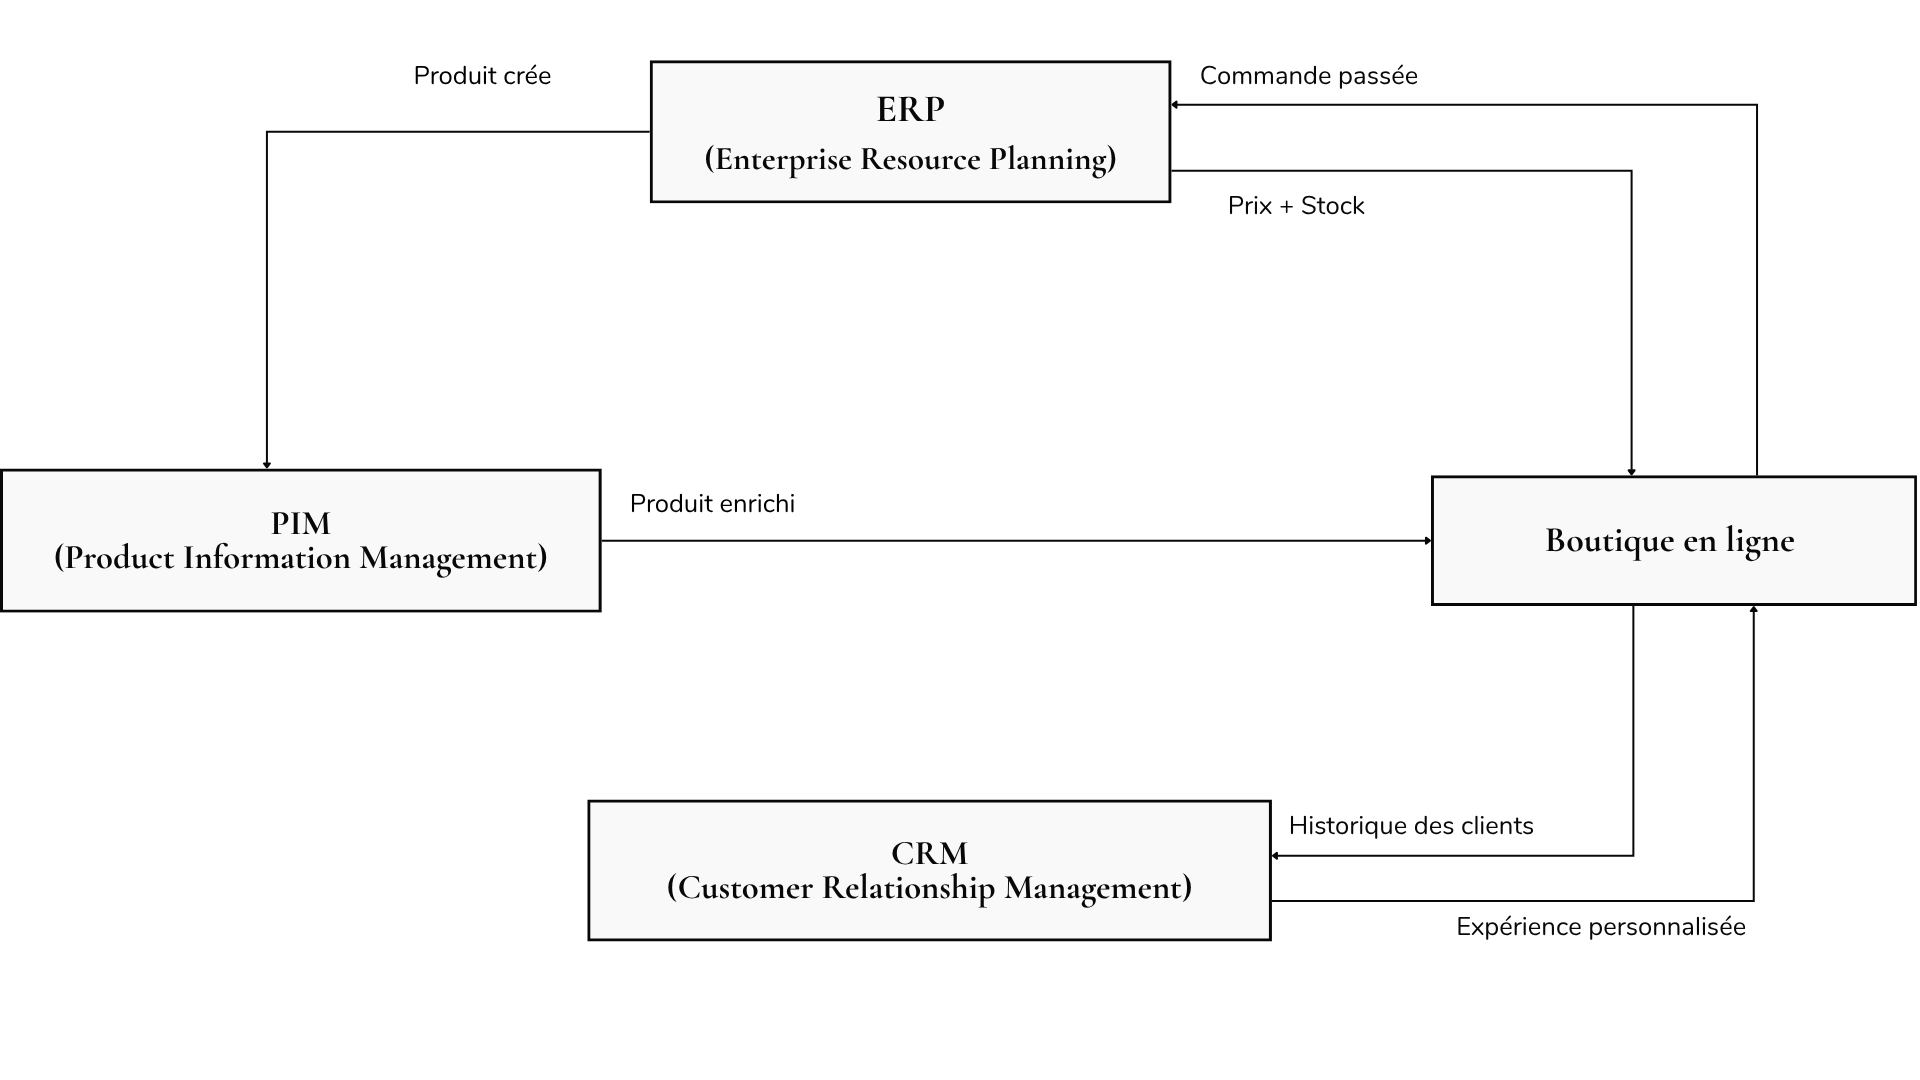
\includegraphics[width=1\textwidth]{images/product.png}
    \caption{Flux de circulation des informations des produits dans l'écosystème e-commerce}
    \label{fig:cycle_vie}
\end{figure}


Le flux commence par la \textbf{création} de la référence de base dans l'ERP. Le produit est ensuite transmis au PIM pour son \textbf{enrichissement} (attributs des produits techniques, médias, traductions). Une fois validées, ces données des produits sont \textbf{publiées} vers SAP Commerce Cloud pour être \textbf{consultées} par les clients sur le Storefront.

Lors de la transaction, SAP Commerce synchronise en temps réel les prix et les stocks avec l'ERP pour finaliser l'achat. Enfin, chaque interaction alimente le CRM pour affiner la connaissance client. La collaboration entre ces systèmes est cruciale : l'ERP assure la fiabilité opérationnelle, le PIM garantit la richesse du contenu, SAP Commerce gère la vente et le CRM valorise les données du client.
\newpage
\section{Cadre général du projet}

\subsection{Contexte}

Dans le cadre de son activité e-commerce, ETANCO gère un catalogue technique très vaste comprenant des fixations, des accessoires ainsi que des systèmes de toiture. Chaque produit est décrit à travers un ensemble riche d’attributs des produits, souvent structurés et dépendants de sa catégorie.
\vspace{0.2cm}

Les données des produits sont principalement saisies et enrichies dans le backoffice SAP Commerce. Elles sont également complétées via des imports ou des mises à jour manuelles réalisées par les équipes métier.
\vspace{0.2cm}

Cependant, malgré les outils existants, certaines informations techniques et commerciales des produits peuvent rester incomplètes ou contenir des erreurs de saisie, ce qui rend les opérations de contrôle complexes avant la mise en ligne sur les plateformes e-commerce.

\subsection{Étude de l’existant}

Actuellement, la publication d’un produit sur le site e-commerce repose sur un processus largement manuel. Lorsqu’un produit est créé ou modifié, plusieurs vérifications doivent être réalisées, notamment le contrôle des noms, des descriptions des produits, des attributs des produits, ainsi que des images associées.
\vspace{0.2cm}

Cette phase se termine par une validation effectuée par le \textit{Product Detail Manager} dans le workflow d’enrichissement intégré à SAP Commerce. Bien que cette étape soit essentielle pour garantir la qualité des informations publiées, elle dépend fortement de l’intervention humaine.
\vspace{0.2cm}

En raison du volume important d’informations à traiter, certaines validations peuvent être partielles. Cela peut entraîner la présence d’erreurs ou d’incohérences dans les informations des produits publiées sur le Storefront.

\section{Problématique et solution proposée}

\subsection{Problématique}

Dans un contexte e-commerce, les clients s’appuient sur les caractéristiques des produits pour prendre leurs décisions d’achat. Toute erreur ou information manquante peut donc avoir un impact direct sur la confiance des clients sur les ventes.
\vspace{0.2cm}

Or, le processus actuel de validation manuelle présente plusieurs limites. Il peut laisser passer certaines anomalies telles que des attributs des produits manquants, des incohérences entre les données ou des problèmes de catégorisation.
\vspace{0.2cm}

Ces problèmes de qualité réduisent la fiabilité des informations publiées. Il devient ainsi nécessaire de fiabiliser le processus d’enrichissement et de validation des données des produits.

\subsection{Solution proposée}

Afin de répondre à cette problématique, la solution proposée consiste à intégrer une couche d’analyse intelligente dans le workflow d’enrichissement de SAP Commerce.
\vspace{0.2cm}

La solution repose sur un service externe accessible via des API REST permettant l’échange des données nécessaires à l’analyse et à la validation. Cette approche vise à renforcer les contrôles de qualité tout en conservant la validation humaine. Elle permet d’automatiser certaines tâches d’enrichissement, telles que la génération de descriptions des produits et la traduction des contenus, ainsi que la normalisation des formats de données.
\vspace{0.2cm}

L’utilisateur conserve un rôle central dans le processus, puisqu’il peut valider ou refuser les suggestions proposées avant leur publication officielle sur le site.
\vspace{0.2cm}

Cette solution contribue à rendre le processus d’enrichissement plus efficace et plus fiable, tout en améliorant la qualité des informations techniques et commerciales des produits publiées en ligne.

\section{Méthodologie de travail adoptée}

Dans le cadre de ce projet, nous avons adopté la méthodologie Agile Scrum, largement utilisée dans le développement logiciel pour sa flexibilité et sa capacité à s'adapter aux besoins évolutifs du projet. Cette approche repose sur un développement itératif et incrémental, permettant de livrer progressivement des fonctionnalités tout en intégrant des retours réguliers des parties prenantes afin d'améliorer continuellement le produit final. Le fonctionnement général de cette méthodologie est présenté dans la Figure~\ref{fig:scrum}.

\begin{figure}[H]
    \centering
    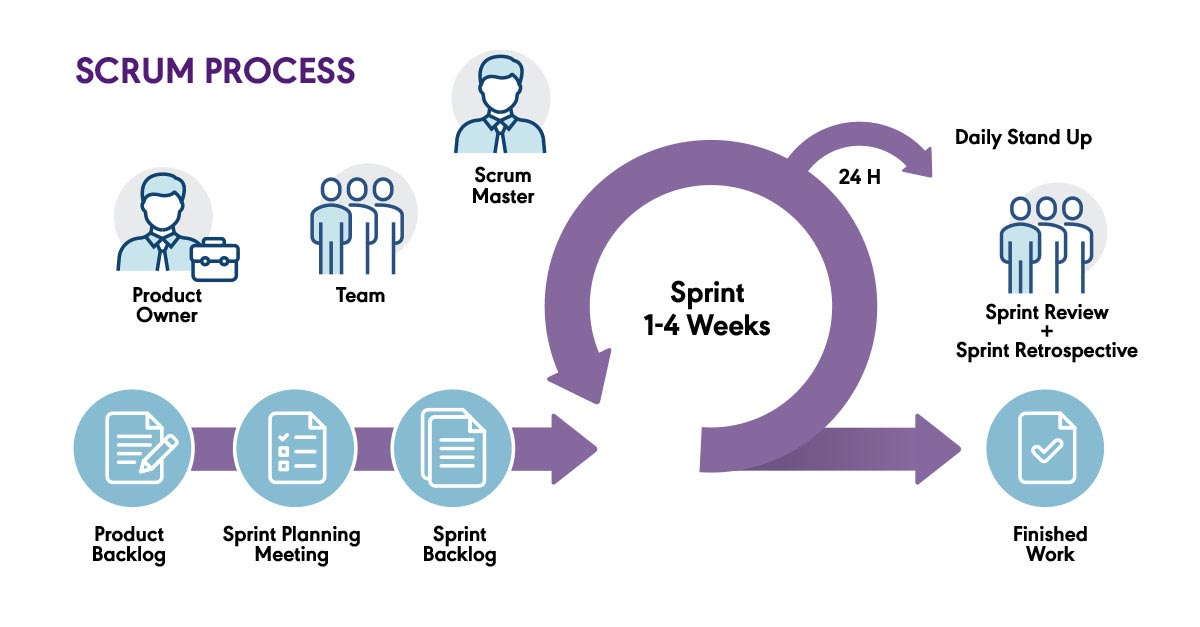
\includegraphics[width=0.75\textwidth]{images/scrum-process.jpg}
    \caption{Principe de la méthodologie Scrum}
    \label{fig:scrum}
\end{figure}

Ce diagramme illustre l'interaction cyclique entre les différents éléments Scrum : la planification initiale, l'exécution des Sprints, les réunions d'examen et les phases de rétrospective. Cette structure permet une amélioration continue tout en assurant une livraison régulière de fonctionnalités opérationnelles.
\newpage
\subsection{Éléments de la méthodologie Scrum}

La méthodologie Scrum repose sur un ensemble d’éléments essentiels qui structurent le processus de développement :

\begin{itemize}

    \item \textbf{Product Backlog :} il s’agit d’une liste priorisée regroupant l’ensemble des fonctionnalités, améliorations et corrections à réaliser sur le produit. Sa gestion est assurée par le Product Owner.

    \item \textbf{Sprint Backlog :} ensemble des tâches sélectionnées à partir du Product Backlog et que l’équipe s’engage à réaliser durant un Sprint.

    \item \textbf{Sprint :} période de développement courte et fixe, généralement de deux à quatre semaines, durant laquelle un incrément fonctionnel du produit est développé.

    \item \textbf{Daily Scrum :} réunion quotidienne de synchronisation permettant de suivre l’avancement, d’identifier les blocages et d’ajuster les priorités.

    \item \textbf{Sprint Review :} réunion organisée à la fin de chaque Sprint afin de présenter les fonctionnalités développées et de recueillir les retours des parties prenantes.

    \item \textbf{Sprint Retrospective :} réunion d’analyse permettant à l’équipe d’identifier les points positifs, les difficultés rencontrées et les axes d’amélioration pour les prochains Sprints.

\end{itemize}

\subsection{Rôles au sein de l’équipe Scrum}

Dans le cadre de ce projet, les rôles Scrum ont été répartis de la manière suivante :

\begin{itemize}

    \item \textbf{Chef de projet technique :} Monsieur Aymen Ellouze, responsable de la coordination technique du projet, de la répartition des tâches et du suivi global de l’avancement.

    \item \textbf{Équipe de développement :} chargée de la conception, de l’implémentation, des tests et de la livraison des différentes fonctionnalités du système.

\end{itemize}
\subsection{Mécanisme de feedback}

Le mécanisme de feedback constitue un élément clé dans l’amélioration continue du projet. Il repose sur des échanges réguliers entre les membres de l’équipe et le chef de projet.

Ainsi, des réunions quotidiennes de type Daily Scrum sont organisées afin de partager l’état d’avancement et d’identifier rapidement les éventuels blocages. En complément, des réunions de suivi sont tenues toutes les une à deux semaines afin de présenter l’avancement global du projet et de valider les fonctionnalités développées.

Ces interactions régulières permettent d’assurer une meilleure adaptation aux besoins du projet et de garantir un alignement constant entre les développements réalisés et les objectifs fixés.
\newpage

\section{Conclusion du chapitre}
Dans ce chapitre, nous avons présenté le cadre général du projet ainsi que l’environnement dans lequel il s’inscrit. Nous avons introduit l’organisme d’accueil DECADE Tunisie et mis en évidence ses activités dans le domaine du commerce en ligne.

Nous avons également analysé le contexte du projet ainsi que le processus existant de gestion des informations des produits, ce qui nous a permis d’identifier les limites actuelles et de définir la problématique.

Enfin, nous avons présenté la solution proposée ainsi que la méthodologie de travail adoptée, basée sur l’approche Agile Scrum, qui permet de structurer efficacement le déroulement du projet et de garantir une progression itérative et contrôlée.